\section{Experiments}
\label{sec:experiments}
\subsection{Available runs and evaluation protocol}
The available artifacts contain configurations, training histories, checkpoints and detection reports for seven runs \cite{comparison,repository}. The custom-run configurations specify CUDA, seed 42, AdamW, step scheduling and gradient clipping. Selected configurations are summarised in Table~\ref{tab:training}; the configured epoch/step limits do not by themselves prove that every full dataset frame was visited in every epoch. The configurations also cap the validation batches used during custom-model training (150 for Faster R-CNN and the RT-DETR variant; 50 for Fast R-CNN and R-CNN). Thus checkpoint selection and the later evaluation reports need not use identical subsets. The YOLO native arguments record 20 epochs, batch size 16, image size 640 and AdamW, while the project's export configuration specifies a stride of five frames for the train and validation splits \cite{yoloargs,yoloconfig}. YOLO's native validation during training and the common evaluator may use different inputs and settings.

\begin{table}[htbp]
\centering
\caption{Selected published training configuration settings. Step caps apply to custom-model epochs.}
\label{tab:training}
\begin{tabular}{lrrrr}
\toprule
Run & Epochs & Batch & Learning rate & Max steps \\
\midrule
Faster R-CNN, scratch & 20 & 8 & 0.001 & 1,000 \\
Faster R-CNN, ImageNet & 15 & 8 & 0.0005 & 1,000 \\
Fast R-CNN, scratch & 10 & 2 & 0.001 & 300 \\
R-CNN, scratch & 10 & 1 & 0.001 & 200 \\
RT-DETR variant, scratch & 20 & 8 & 0.0005 & 1,000 \\
YOLOv8n, fine-tuned & 20 & 16 & 0.001 & --- \\
\bottomrule
\end{tabular}
\end{table}

Detection performance is measured with the project evaluator using COCO-style average precision (AP) at IoU 0.50 and mean AP over IoU 0.50--0.95. Precision and recall use confidence 0.25, class-aware one-to-one matching and IoU 0.50, with the ignore policy described in Section~\ref{sec:dataset}. All metrics in the published comparison CSV are labelled \texttt{val}, and no test-set result is asserted here. The evaluation script limits Fast R-CNN and R-CNN batches; the resulting reports each contain 400 frames. Other reports contain all 10,260 frames listed in the validation manifest \cite{evaluationcode,evalscript,comparison}.

\subsection{Validation detection results}
Table~\ref{tab:full} presents the five reports with the full validation frame count. The values are rounded to three decimals from the published CSV. AP depends on confidence-ranked predictions over the evaluator's thresholds, whereas the precision and recall columns are reported at a fixed confidence of 0.25. Initialization, architecture, data sampling and training budgets differ, so the table is an empirical comparison of these runs rather than a controlled ablation.

\begin{table}[htbp]
\centering
\caption{Detection reports on the 10,260-frame validation split. AP values are fractions.}
\label{tab:full}
\begin{tabular}{lrrrr}
\toprule
Run & AP$_{50}$ & AP$_{50:95}$ & Precision & Recall \\
\midrule
Faster R-CNN, scratch & 0.642 & 0.416 & 0.828 & 0.829 \\
Faster R-CNN, ImageNet & 0.719 & 0.507 & 0.736 & 0.805 \\
RT-DETR-inspired, scratch & 0.367 & 0.238 & 0.386 & 0.826 \\
YOLOv8n, COCO & 0.365 & 0.259 & 0.767 & 0.670 \\
YOLOv8n, fine-tuned & 0.750 & 0.564 & 0.825 & 0.907 \\
\bottomrule
\end{tabular}
\end{table}

The corresponding reports for Fast R-CNN and R-CNN cover only 400 validation frames (Table~\ref{tab:partial}). Both JSON files mark AP for \texttt{bus} and \texttt{others} as unavailable ($-1$), so their aggregate AP does not represent the same set of evaluable classes as the full-split reports. They are reported separately because a different number and potentially different distribution of frames invalidate a direct ranking against Table~\ref{tab:full}. They may also differ from a full-split estimate even when the same metric code is used.
\begin{table}[htbp]
\centering
\caption{Partial validation reports: 400 frames per run.}
\label{tab:partial}
\begin{tabular}{lrrrr}
\toprule
Run & AP$_{50}$ & AP$_{50:95}$ & Precision & Recall \\
\midrule
Fast R-CNN, scratch & 0.409 & 0.267 & 0.667 & 0.335 \\
R-CNN, scratch & 0.132 & 0.053 & 0.458 & 0.151 \\
\bottomrule
\end{tabular}
\end{table}

\subsection{Training curves and runtime}
The published project figure summarises training losses and per-epoch validation AP (Fig.~\ref{fig:curves}) \cite{curves}. We compared all 95 rows of its companion CSV against the original per-epoch logs and the YOLO training CSV, including the plotted loss and AP fields, within the CSV's five-decimal rounding; no field mismatch was found. The script combines distinct evaluation subsets: the recorded custom-model validation logs contain 1,200 frames per epoch for Faster R-CNN and the RT-DETR variant, 100 for Fast R-CNN and 50 for R-CNN. The YOLO series comes from its native training results on the exported validation data configured with stride five. In the first and last logged Faster R-CNN epochs, the per-class AP array reports the \texttt{others} class as unavailable ($-1$); in the corresponding Fast R-CNN and R-CNN logs, both \texttt{bus} and \texttt{others} are unavailable. The plotted values must therefore not be interpreted as performance over the same frames or the same set of evaluable classes \cite{plotcode,curveaudit}. Loss magnitudes and validation procedures are not directly comparable across architectures; YOLO's native validation is not the same artifact as the shared-evaluator results in Tables~\ref{tab:full} and \ref{tab:partial}. Curves show the recorded runs' evolution, not uncertainty across independent seeds.
\begin{figure}[htbp]
\centering
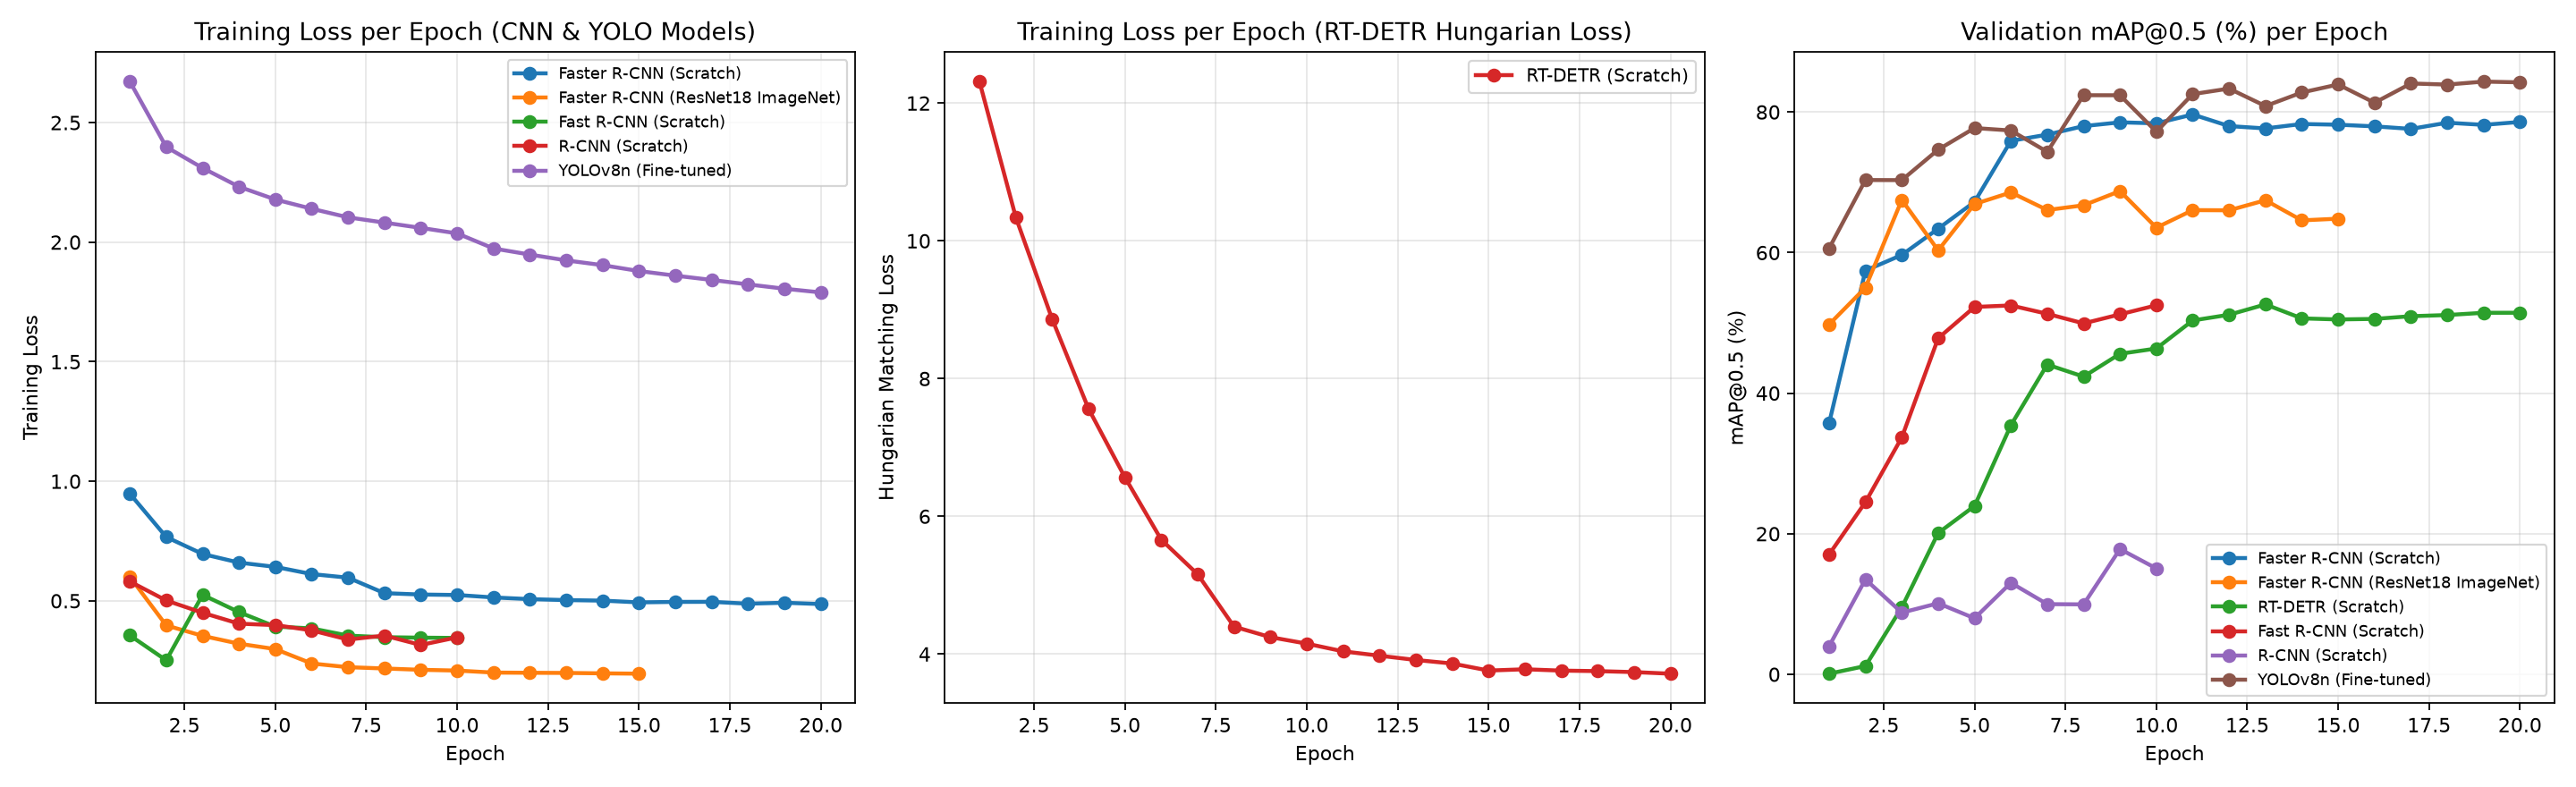
\includegraphics[width=.76\textwidth,trim=0 0 867pt 0,clip]{figures/training_loss_and_map_curves.png}
\caption{Published training losses for the R-CNN family and YOLO, enlarged from the original composite plot. The loss functions differ, so their magnitudes are not directly comparable.}
\label{fig:curves}
\end{figure}
\begin{figure}[htbp]
\centering
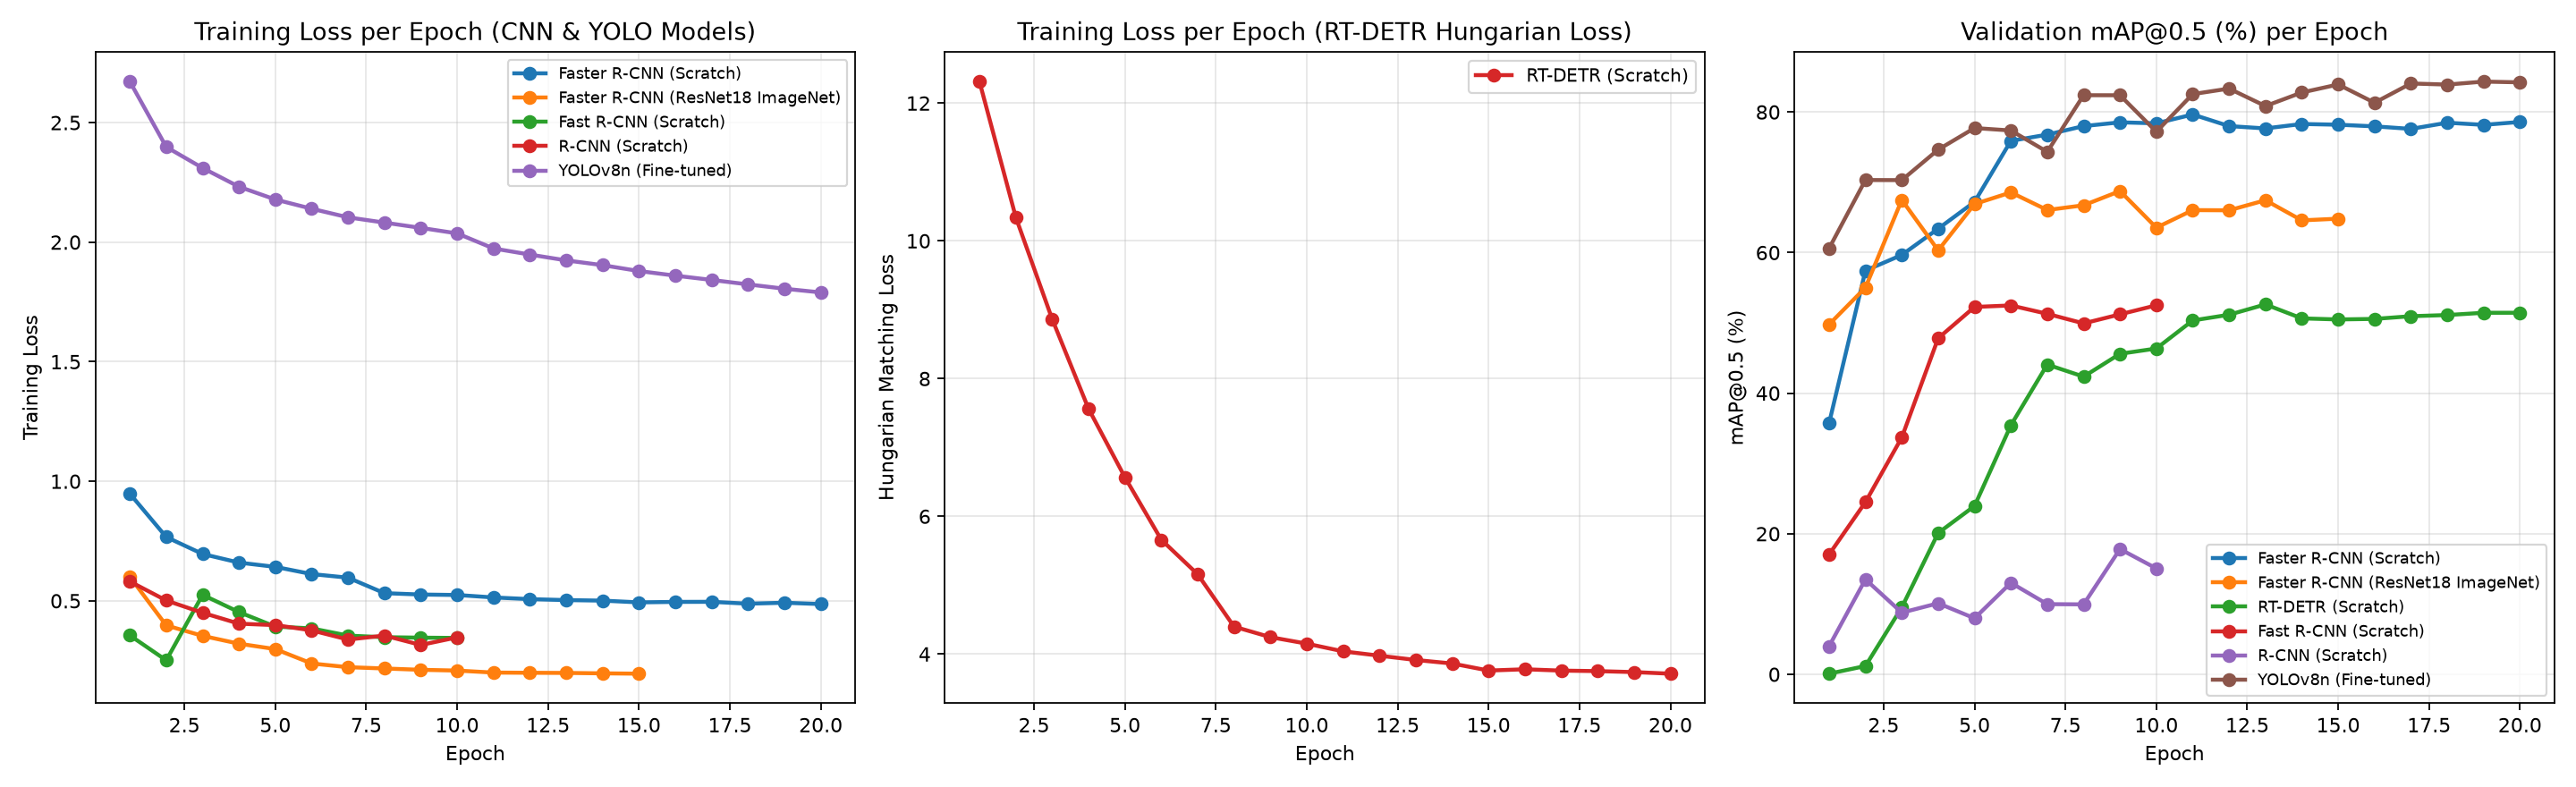
\includegraphics[width=.76\textwidth,trim=433pt 0 434pt 0,clip]{figures/training_loss_and_map_curves.png}
\caption{Published RT-DETR training loss, enlarged from the original composite plot. The original title calls it Hungarian matching loss, but the plotting script uses the total logged training loss; matching is an assignment step.}
\end{figure}
\begin{figure}[htbp]
\centering
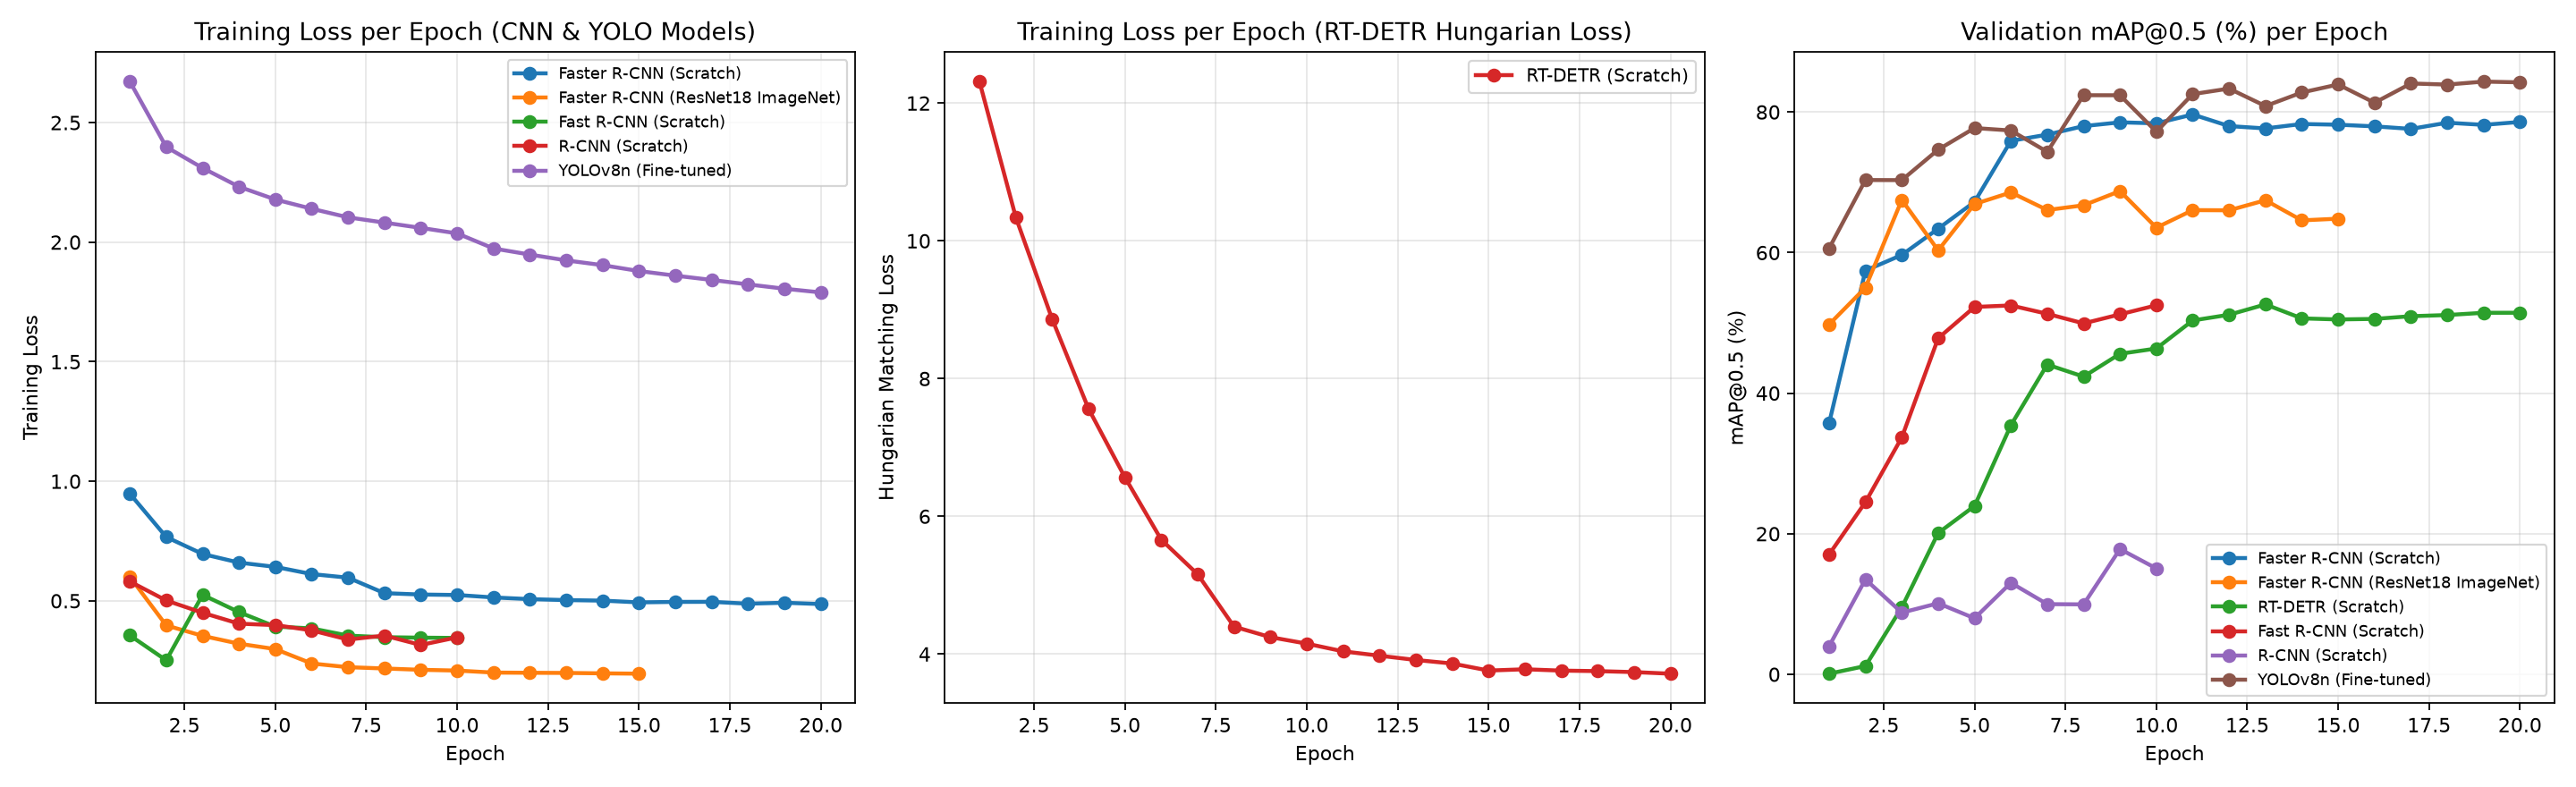
\includegraphics[width=.76\textwidth,trim=867pt 0 0 0,clip]{figures/training_loss_and_map_curves.png}
\caption{Published validation curves, enlarged from the original composite plot. The series use different numbers of frames and evaluable classes and do not constitute a common-split comparison.}
\end{figure}

The comparison file also includes prediction latency and FPS, for example 7.85 ms per image for scratch Faster R-CNN and 16.36 ms for fine-tuned YOLOv8n. The evaluator times calls to the detector adapter, not the complete decode--detect--track--render pipeline. The inspected results do not identify the GPU model or fully specify timing conditions; consequently these numbers should be treated as run-specific measurements, not general deployment or hardware-independent benchmarks \cite{evaluationcode,comparison}.
